% Manual_MILP_BH_en.txt
% ver1: Sept 7, 2020

\documentclass[11pt, titlepage, dvipdfmx, twoside]{article}
\linespread{1.1}

\usepackage{amsfonts}
\usepackage{amssymb}
\usepackage{amsmath}
\usepackage{amsthm}
\newtheorem{theorem}{Theorem}
\newtheorem{lemma}[theorem]{Lemma}
\usepackage{enumitem}
\usepackage{geometry}
\geometry{left=2.5cm, right=2.5cm, top=2.5cm, bottom=2.5cm}

\usepackage{mathtools}
\usepackage{comment}
\usepackage[dvipdfmx]{graphicx}
\usepackage{float}
\usepackage{framed}
\usepackage{graphicx}
\usepackage{subcaption}
\usepackage{listings}
\usepackage{color}
\usepackage{url}
 
\definecolor{codegreen}{rgb}{0, 0.6, 0}
\definecolor{codegray}{rgb}{0.5, 0.5, 0.5}
\definecolor{codepurple}{rgb}{0.58, 0, 0.82}
\definecolor{backcolour}{rgb}{0.95, 0.95, 0.92}

\newcommand{\tname}{6Hc} 
%%  target name used for the example 

\newcommand{\dist}{\mathrm{dist}}

\title{\Huge{Inferring an Acyclic Graph with Bounded Branch-Height
			  from a Trained ANN using MILP}}

\begin{document}

% The following makeatletter must be after begin{document}
\makeatletter 
\let\c@lstlisting\c@figure
\makeatother

\date{\today}

\maketitle

% \cleardoublepage

\thispagestyle{empty}
\tableofcontents
\clearpage

\pagenumbering{arabic}


\section{Outline}
\label{sec:Intro}

This note explains how to use an implementation of a mixed-integer
linear programming (MILP) formulation that can infer
a vector of graph descriptors given a target value and the 
weights and bias values of a trained artificial neural network (ANN).

The MILP is implemented in Python, 
using the PuLP modeling module of the 
COIN-OR package~\cite{PuLP1,PuLP2,PuLP3,PuLP4}.

To begin with, we give a list of the files that accompany this note.

\begin{itemize}

\item Folder {\tt source\_code}\\
A folder containing three python scripts that implement
an MILP formulation for inferring feature vectors
of acyclic chemical graphs from a trained ANN,
and files containing minimum and maximum values
of each descriptor, used for setting the applicability domain
in the MILP formulation.

\begin{itemize}

\item {\tt ann\_inverter.py}\\
An implementation of an MILP formulation 
for the Inverse problem on  ANNs~\cite{AN19}.

\item {\tt acyclic\_graphs\_MILP.py}\\
A python script that contains functions to initialize the variables and prepare 
the constraints for an MILP
formulation for inferring acyclic graphs with a bounded branch-tree height~\cite{acyclic_BH}.

\item {\tt infer\_acyclic\_graphs.py}\\
A python script that prepares the data and executes 
the MILP formulation for given input data.
Further details on the use of this script
are given in Section~\ref{sec:Exp}.

\item {\tt AD\_min.txt}\\
A file containing minimum values over all descriptors, 
used to set the applicability domain
part of the MILP constraints.

\item {\tt AD\_max.txt}\\
A file containing maximum values over all descriptors, 
used to set the applicability domain
part of the MILP constraints.
\end{itemize}

\item  Folder {\tt test\_files}\\
A folder containing data from a trained ANN.
For each of the files, the data format is explained in Section~\ref{sec:InOut},
and an actual example is given in Section~\ref{sec:Exp}.
%
\begin{itemize}
\item {\tt \tname\_desc.csv}\\
A comma-separated value file containing descriptors
used in the training of the ANN.

\item {\tt \tname\_biases.txt}\\
A file containing the values of the biases of a trained ANN.

\item {\tt \tname\_weights.txt}\\
A file containing the values of the weights of a trained ANN.

\end{itemize}
\end{itemize}

The remaining of this note is organized as follows.
Section~\ref{sec:Pre} gives an explanation 
of the used terms and notation.
%
Section~\ref{sec:InOut} explains the 
input and output data of the program,
and Sec.~\ref{sec:Exp} gives a concrete
example of input data and the results form the computation.

% \newpage

\section{Terms and Notation}
\label{sec:Pre}
%
This section explains the terms and notation used in this note.


\begin{itemize}

\item {\bf Feature vector}\\
%
A {\em feature vector} stores numerical values of certain parameters,
called {\em descriptors}.
In this work, we choose graph-theoretical descriptors, such as number of 
non-hydrogen atoms, number of vertices of certain degree, etc.

\item {\bf Artificial neural network}\\
%
Artificial neural networks are one of the methods in machine learning.
They provide a means to construct a correlation function between 
pairs of feature vectors as input and target data as output.


\item {\bf Input, hidden, and output layer}\\
%
We deal with the multilayer perceptron model 
of feed-forward neural networks.
These neural networks are constructed of several {\em layers}.
First comes the \emph{input layer}, where each neuron takes as input
one value of the feature vector.
Next come the \emph{hidden layers}, where the 
values from the input layer are propagated in a feed-forward manner,
such that each node in one layer is connected to all the nodes of the next layer. 
Finally, the output is deliver at the \emph{output layer}.
We deal with predicting the value of a single target,
and hence we assume that the output layer comprises a single node.

\item {\bf Weights}\\
%
Each edge connecting two nodes in an ANN is assigned a real value,
called a \emph{weight}.
Part of the \emph{learning} process of ANNs is to determine values for each of the weights
based on known pairs of feature vectors and target values.

\item {\bf Biases}\\
Each node of an ANN except for the nodes in the input layer
is assigned a real value, called a {\em bias},
which, just like the edge weights, is determined through the learning process.


\item {\bf Activation function}\\
%
In an ANN, each node produces an output as a function, called the \emph{activation function}, 
of its input.
We assume that each node has the Rectified Linear-Unit (ReLU) function 
as its activation function,
which can be expressed exactly in the MILP formulation
for the inverse problem on ANNs~\cite{AN19}.
%https://scikit-learn.org/stable/modules/generated/sklearn.neural\_network.MLPRegressor.html

\item {\bf Mixed-Integer Linear Programming (MILP)}\\
%
A type of a mathematical programming problem
where all the constraints are given as linear expressions, and
some of the decision variables are requested to take
only integer values.
For more details, see any standard reference, e. g.~\cite{LP}.


\item {\bf Graph} \\
An abstract combinatorial construction comprising
a finite set of {\em vertices}, and a finite set of {\em edges},
where each edge is a pair of vertices.
We treat {\em undirected} graphs,
i. e., graphs where edges are unordered pairs of vertices.
For more information, see e. g.~\cite{graph}.

% \item {\bf Directed Tree} \\
% %%% Is this term used anywhere?
% % 長さ1以上の閉路を持たず連結である有向グラフを有向木と呼ぶ.
% % 有向木において枝$(u,v)$が存在するとき,$u$は$v$の親,$v$を$u$の子と呼ぶ.
% % 詳細については参考文献~\cite{graph}を参照すること.


% % \item {\bf Scheme Graph}\\
% %%% Is this term used anywhere?


\end{itemize}

% \newpage

\section{The Program's Input and Output}
\label{sec:InOut}

This section explains the format of the input and the output of the program.
Section~\ref{sec:section3_1} illustrates an example of the program's input format,
and Section~\ref{sec:section3_2} gives a concrete computational example.
Following, Section~\ref{sec:section3_3}illustrates an example of the program's output format,
and Section~\ref{sec:section3_4} gives a concrete computational example.


\subsection{Program Input}
\label{sec:section3_1}

This section gives an explanation of the input to the program.

First and foremost comes the target value for which we wish to infer 
a chemical graph based on a trained ANN.

Next come several parameters pertaining to the 
graph structure that we seek to infer: \\
~~~~- the number of vertices $n^*$, \\
~~~~- the diameter ${\rm dia^*}$, \\
~~~~- branch-height parameter $k^*$, \\
~~~~- maximum degree $d_{\max} \in \{3, 4\}$ of a vertex in the target graph,\\
~~~~- the $k^*$-branch-leaf-number ${\rm bl}_{k^*}$, and \\
~~~~- the $k^*$-branch-height ${\rm bh}_{k^*}$.

Next comes a choice of MILP solver program to be used.
We can choose \\
~~~~- 1: CPLEX, a commercial MILP solver~\cite{cplex}. \\
(Note, in this case the parameter {\tt CPLEX\_PATH} in the file {\tt infer\_acyclic\_graphs.py}
must be set to the correct path of the CPLEX program executable file.) \\
~~~~- 2: CBC, a free and open-source MILP solver that comes together with the PuLP plugin for python~\cite{PuLP1}.

Finally
the input requires three textual files containing \\
~~~~- the descriptor names, in csv format \\
~~~~- the weights and biases of a trained ANN in textual format.\\
For a common prefix {\tt TT} which the program accepts as a command-line parameter,
these files must be saved with file names {\tt TT\_desc.csv}, 
{\tt TT\_weights.txt} and {\tt TT\_biases.txt} for the files containing
the descriptor names, the weights, and the biases of a trained ANN, respectively.



\subsection{Input Data Format}
\label{sec:section3_2}

This section presents an actual example of an input instance of the program.
In particular, we give a concrete example of the three input files
mentioned in Section~\ref{sec:section3_1}.

The purpose of this program is to calculate a feature vector that will produce a desired output from a 
given trained ANN.
Figure~\ref{fig:sample} gives an example of a trained ANN.


\begin{figure}[H]
  \centering
  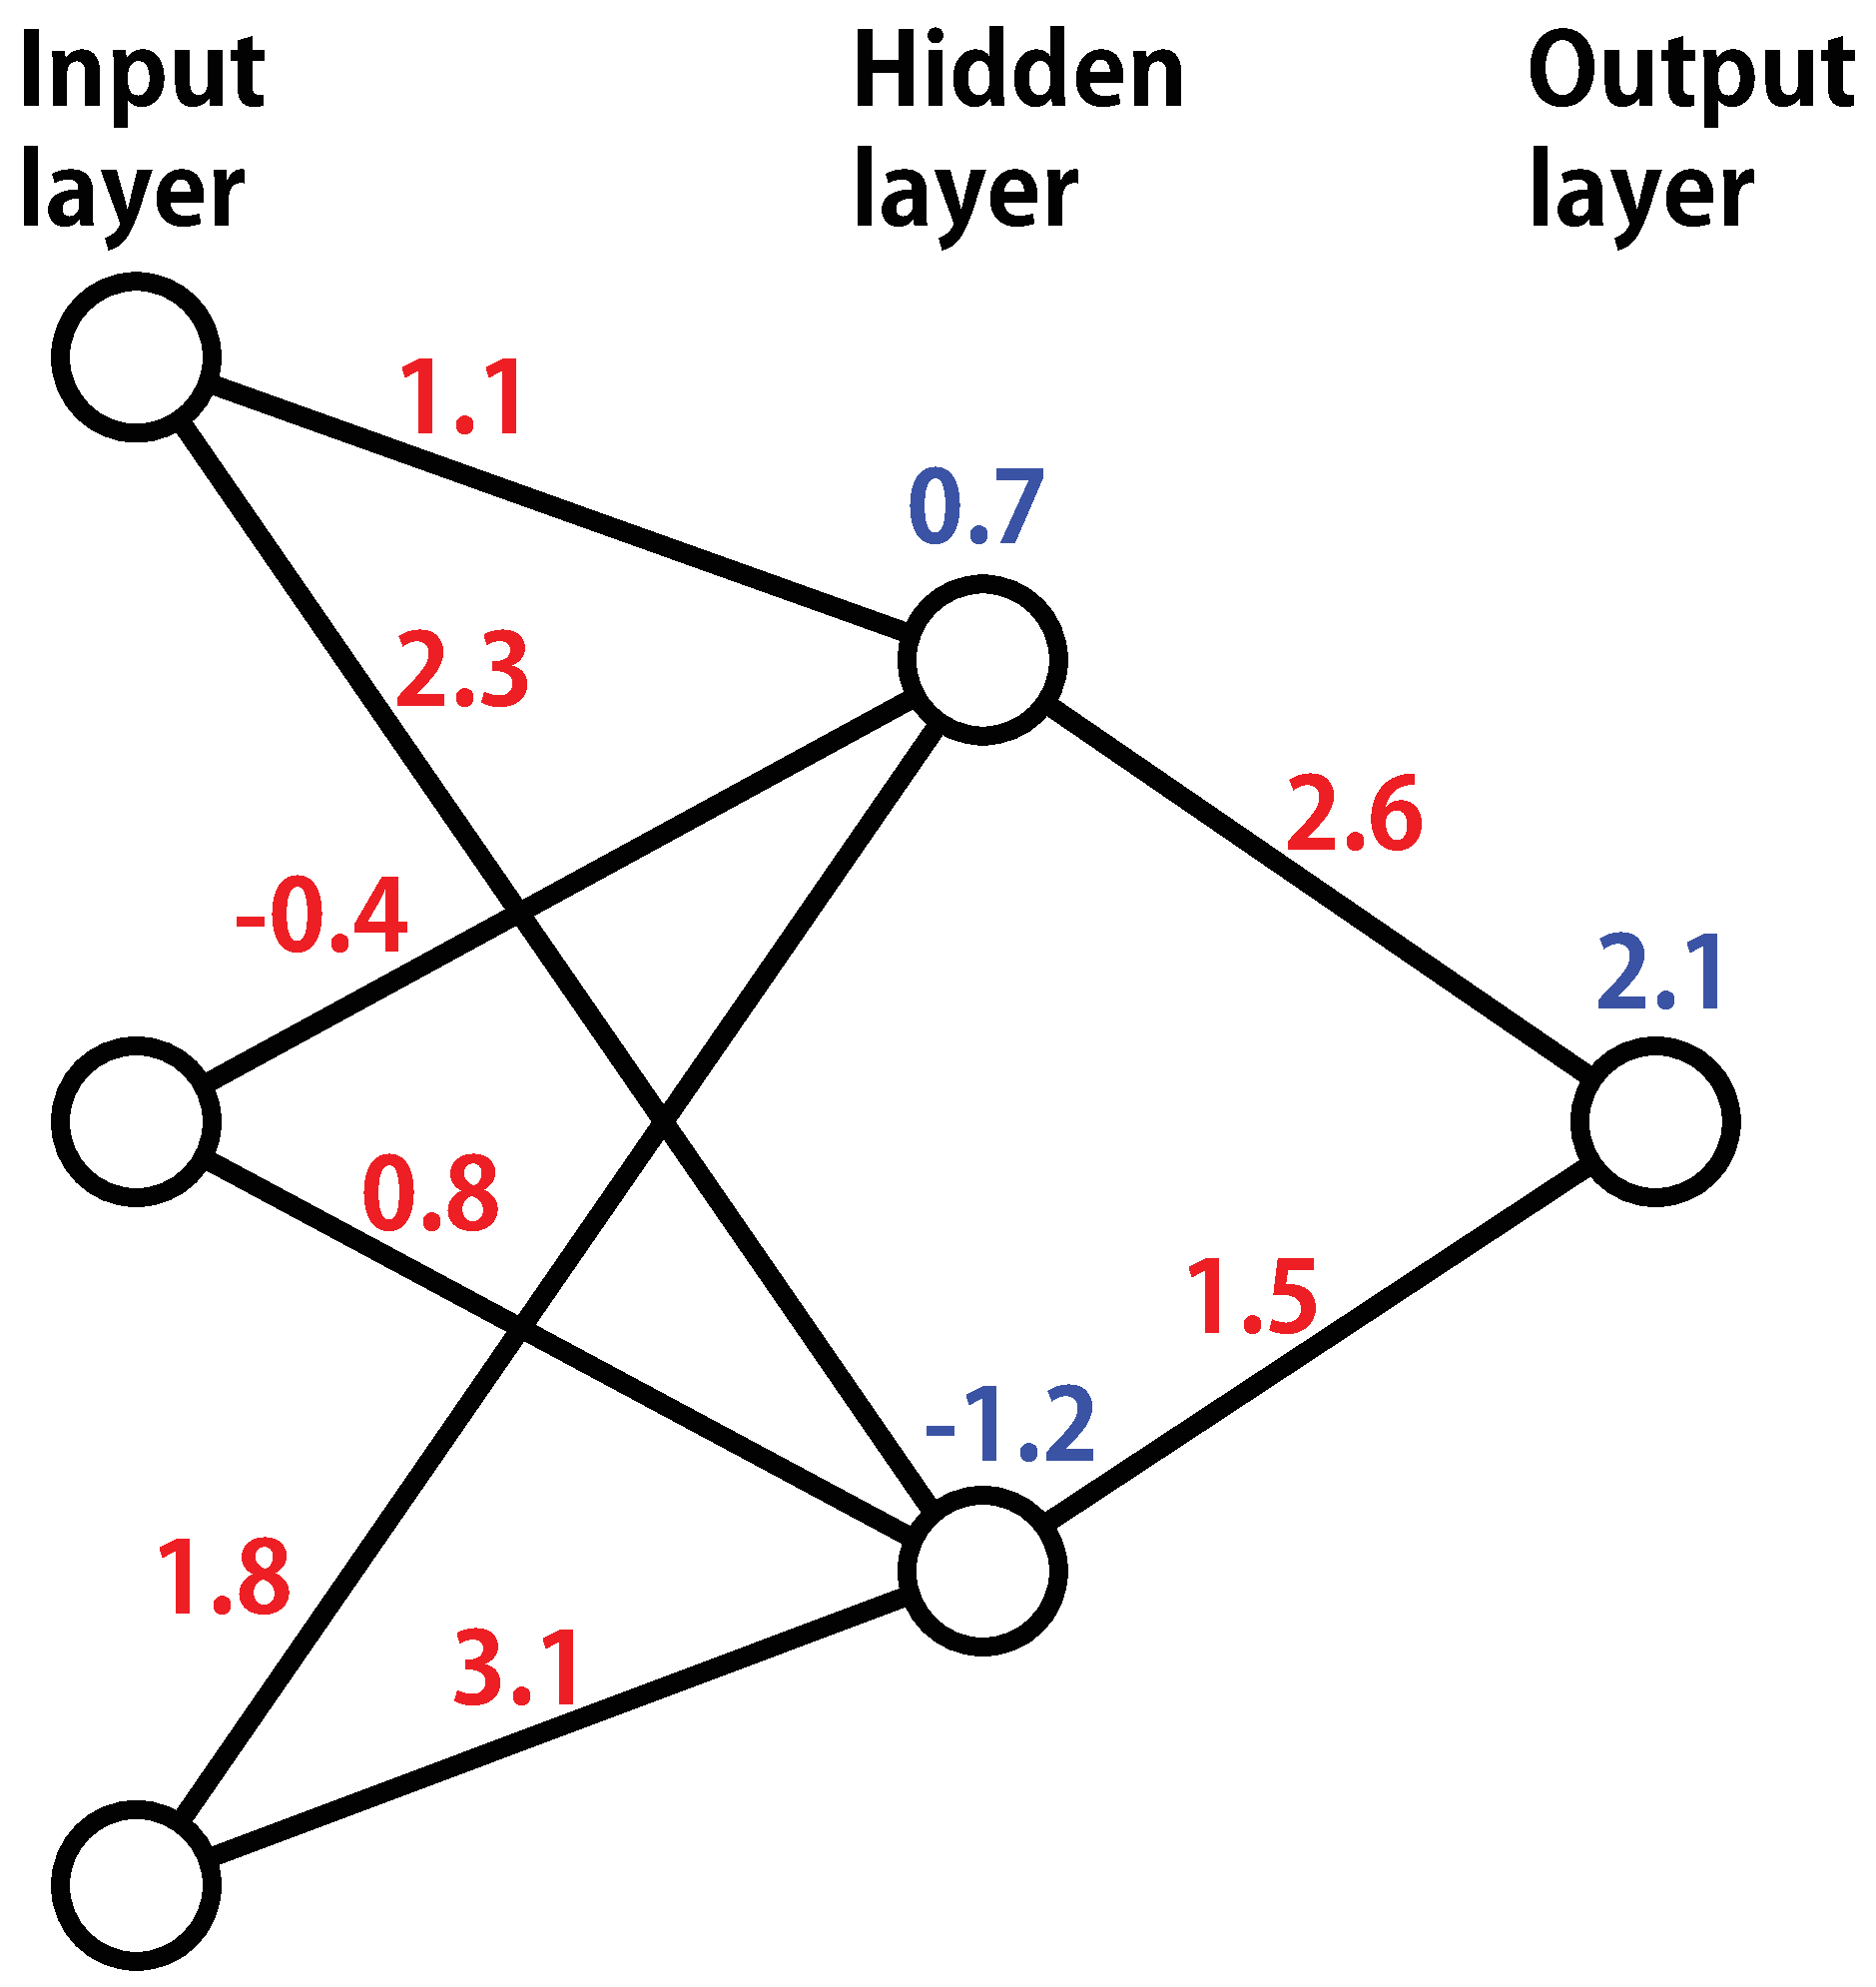
\includegraphics[width=0.5\textwidth]{./fig/ANN_sample_en}
  \caption{An example of a trained ANN.
		      The ANN's weights are given in red numbers, and
		      its biases in blue.
		    }
  \label{fig:sample}
\end{figure}


The information on the trained ANN is written in two text files, containing the information
on the ANN's weights and biases, respectively.
First, we give the structure of the file that contains the information on the ANN's weights.
The first line of this text file contains the information on the ANN's architecture, i. e., 
the number of nodes in each of its layers.
From the second row and onward
follows the information on the 
weights in the ANN.
Each row contains the weights of the edges that are incident to one node of the ANN,
first of the nodes in the input layer, and then for the nodes of the hidden layers.
Following is a textual example for the ANN given in Fig.~\ref{fig:sample}.

\bigskip

\begin{oframed}
{\bf Organization of the text file containing weight data}\\\\
%\bigskip\bigskip
3 2 1\\
1.1 2.3\\
-0.4 0.8\\
1.8 3.1\\
2.6\\
1.5\\
\end{oframed}

\bigskip

Next, comes the text file with the information on the ANN's biases.
二つ目はバイアスのデータが含まれたテキストファイルである.
各行にバイアスの値が記入されている.
記入されている順番は,入力層の一つ目のノードから最後のノード,中間層の一つ目のノードから最後のノード,出力層のノードである.
図~\ref{fig:sample}のバイアスのデータを記入したテキストファイルは以下のようになる.

\bigskip

\begin{oframed}
{\bf Bias values}\\\\
%\bigskip\bigskip
0.7\\
-1.2\\
2.1\\
\end{oframed}

\bigskip

最後に,特徴ベクトルのデータが含まれたテキストファイルの形式について説明する.
このテキストファイルでは,一行目に特徴ベクトルの構成要素が記入されている.
二行目以降の各行に特徴ベクトルの数値データが記入されている.
このテキストファイルの具体例を以下に示す.

\bigskip

\begin{oframed}
{\bf 特徴ベクトルのデータ形式}\\\\
%\bigskip\bigskip
CID,n,M,C,O,H,C1O,C2O,C1C,C2C,\#degree1,\#degree2,\#degree3,\#degree4,\#degree5,\\
\#degree6,\#double\_bond,\#triple\_bond,Diameter,bc\_121,bc\_122,bc\_123,bc\_131,
bc\_132, \\bc\_141,bc\_221,bc\_222,bc\_223,bc\_231,bc\_232,bc\_241,bc\_331,bc\_332,bc\_341,bc\_441,2-branch\_height,2-branch\_number\\
7778,13,126.154,11,2,20,2,1,8,1,4,7,2,0,0,0,2,0,0.769231,0,1,0,3,0,0,5,0,0,2,1,0,0,0,0,0,1,2
\\
86749,11,123.636,10,1,20,1,0,8,1,5,4,1,1,0,0,1,0,0.636364,1,0,0,2,0,2,2,0,0,0,1,2,0,0,0,0,1,2
\\
5282109,13,126.154,11,2,18,2,1,7,2,4,7,2,0,0,0,3,0,0.769231,0,1,0,3,0,0,5,0,0,1,2,0,0,0,0,0,1,2
\\
5319723,11,123.636,10,1,16,1,0,6,3,4,5,2,0,0,0,3,0,0.727273,1,1,0,1,1,0,2,0,0,3,1,0,0,0,0,0,1,2
\\
\hspace{5mm}\vdots
\\
\hspace{5mm}\vdots

\end{oframed}

\bigskip



\subsection{プログラムの出力}
\label{sec:section3_3}

この節では,プログラムの出力情報について説明する.
このプログラムでは,与えられた活性値を満たすような特徴ベクトルが存在する場合は
その特徴ベクトルを出力する.
そなような特徴ベクトルが存在しない場合は,存在しないと出力する.
次の節で出力結果の形式について説明する.

\subsection{出力データの形式}
\label{sec:section3_4}

この説では,計算機上でプログラムを実行した際に出力されるデータ形式について説明する.


まず特徴ベクトルのそれぞれの特徴量が各行に表示される.
次に,化学グラフの情報が表示される.
各節点が対応する原子が表示される.
それぞれの節点には番号が割り振られている.
そして,各節点の隣接リストが表示される.
リストに含まれる節点番号の原子に結合が存在することを表しており,括弧内の値は結合の多重度を表している.
出力結果の具体例を以下に示す.

\bigskip

\begin{oframed}
{\bf ターミナル上の出力結果のデータ形式}\\\\
%\bigskip\bigskip
Status:Optimal \\ 
Initializing Time: 3.8026208877563477 \\ 
Solving Time: 20.04114603996277

\end{oframed}

さらに,ターゲット値及び他の引数に応じての名前が変わる{\tt sdf}ファイルが結果として作ります.
このファイルは世界中水準の{\tt sdf}フォーマットで一つのグラフを格納しています.



\section{プログラムの実行と計算例}
\label{sec:Exp}

この節ではプログラムの実行例を説明する.
ここではプログラム{\tt infer\_acyclic\_graphs.py}の実行方法と結果の具体例を示す.

% % \subsection{Computing environment}
% % The following results are from executing the program on a
% % MacBook Air (13-inch model from 2017), with 
% %  Intel Core i5 processor running at 1.8 GHz and 8 GB of memory.
 


\subsection{実行方法}
\label{sec:Exp_1}

まず,ターミナル上でディレクトリをフォルダsource\_codeに変更する.
このプログラムを実行するためには,ターミナル上で以下のコマンドを実行する.\\

{\tt python3 infer\_acyclic\_graphs.py target value 
$n^\ast$ ${\rm dia}^\ast$ $k^\ast$ $d_{\max}$ bn$_{k^\ast}$  bh$_{k^\ast}$ solver\_type property}\\

ここで, solver\_type=1の時,ソルバーとしてCPLEXが使われる. solver\_type=2の時,ソルバーとしてCoin-ORが使われる.
例えば,
target value=1900 $n^\ast$=15 ${\rm dia}^\ast$=10 $k^\ast$=2 $d_{\max}$=3 bn$_{k^\ast}$=3 bh$_{k^\ast}$=2 solver\_type=1  
propertyがretention timeとすれば,コマンドが以下のようになる.\\

{\tt python3 infer\_acyclic\_graphs.py 1900 15 10 2 3 3 2 1 rt}\\

このコマンドを実行すると計算が実行され,計算結果が出力される.


\begin{oframed}
{\bf 出力データの形式}\\\\
%\bigskip\bigskip
{\tt 2\\
C 120 4 5 8\\
O 160 2 2 0\\
3\\
C C 2 0 3\\
C O 1 4 0\\
C C 1 2 5\\
0 6\\
4 1\\
3 1\\
0 0\\
10\\
3\\
1 2 1 0 1\\
1 2 2 0 0\\
1 2 3 0 0\\
1 3 1 0 2\\
1 3 2 0 3\\
1 4 1 0 0\\
2 2 1 2 0\\
2 2 2 0 0\\
2 2 3 0 0\\
2 3 1 4 1\\
2 3 2 0 0\\
2 4 1 0 0\\
3 3 1 0 1\\
3 3 2 0 0\\
3 4 1 0 0\\
4 4 1 0 0\\}
\end{oframed}


この具体例を用いて,各行の内容を説明する.
数値例とそれぞれの内容の対応を表~\ref{tab:InputFormat}に示す.

\bigskip
\begin{table}[H]
\begin{center} \caption{入力するテキストファイルの読み方}
\label{tab:InputFormat}
  \begin{tabular}{l|l}
  数値例 & 内容\\ \hline \hline
{\tt  2} & 原子の種類\\ \hline
{\tt  C 120 4 5 8} & 原子のシンボル,質量の十倍,価数,原子の内部節点数,原子の外部節点数\\
{\tt  O 160 2 2 0} & \\ \hline
{\tt  3} & 原子結合の種類 \\ \hline
{\tt  C C 2 0 3} & \\
{\tt  C O 1 4 0} &  原子結合(原子,原子,多重度),内部原子結合の数,外部原子結合の数 \\
{\tt  C C 1 2 5} & \\ \hline
{\tt  0 6} & 度数が1の内部節点数,度数が1の外部節点数 \\ 
{\tt  4 1} & 度数が2の内部節点数,度数が2の外部節点数 \\
{\tt  3 1} & 度数が3の内部節点数,度数が3の外部節点数 \\
{\tt  0 0} & 度数が4の内部節点数,度数が4の外部節点数 \\ \hline
{\tt  10} & 直径 \\ \hline
{\tt  3} & 度数の上限 \\ \hline
{\tt  1 2 1 0 1} & \\
{\tt  1 2 2 0 0} & \\
{\tt  1 2 3 0 0} & \\
{\tt  1 3 1 0 2} & \\
{\tt  1 3 2 0 3} & \\
{\tt  1 4 1 0 0} & \\
{\tt  2 2 1 2 0} & 度数結合(度数,度数,多重度),内部度数結合の数,外部度数結合の数 \\
{\tt  2 2 2 0 0} & \\
{\tt  2 2 3 0 0} & \\
{\tt  2 3 1 4 1} & \\
{\tt  2 3 2 0 0} & \\
{\tt  2 4 1 0 0} & \\
{\tt  3 3 1 0 1} & \\
{\tt  3 3 2 0 0} & \\
{\tt  3 4 1 0 0} & \\
{\tt  4 4 1 0 0} & \\ \hline
  \end{tabular}
\end{center}
\end{table}

%出力結果のフォーマットについては第~\ref{sec:section3_3}節および第\ref{sec:section3_4}節を参照すること.

% \subsection{計算例}
% \label{sec:Exp_2}
% 
% この節では,プログラムを実行した結果の具体例を説明する.
% 今回は化学活性Heat of Atomizationのデータを使って計算を行った.
% また他の数値は以下のように設定した.
% 
% 
% \bigskip



\begin{thebibliography}{99}
  \bibitem{AN19} 
    T.~Akutsu and H.~Nagamochi.
    A Mixed Integer Linear Programming Formulation to Artificial Neural Networks,
    in Proceedings of the 2019 2nd International Conference on Information Science and Systems,
    pp.~215--220, https://doi.org/10.1145/3322645.3322683.
    
  \bibitem{acyclic_BH}
	  N.~A.~Azam, J.~Zhu, Y.~Sun, Y.~Shi, A.~Shurbevski, L.~Zhao, H.~Nagamochi and T.~Akutsu.
	  A Novel Method for Inference of Acyclic Chemical Compounds with Bounded Branch-height Based on Artificial Neural Networks and Integer Programming.
	  
%   \bibitem{graph} 茨木俊秀,永持仁,石井利昌.グラフ理論ー連結構造とその応用ー.朝倉書店,2010. 
%   
%   \bibitem{LP} 福島雅夫.数理計画入門.朝倉書店,2012. 
  \bibitem{LP} J.~Matousek and B.~G\"{a}rtner.
			      Understanding and Using Linear Programming. Springer, 2007.
			      
  \bibitem{graph} M.~S.~Rahman.
			      Basic Graph Theory. Springer, 2017.
  
  \bibitem{PuLP1} A Python Linear Programming API, \url{https://github.com/coin-or/pulp}.
  
  \bibitem{PuLP2} Optimization with PuLP, \url{http://coin-or.github.io/pulp/}.
  
  \bibitem{PuLP3} The Python Papers Monograph, \url{https://ojs.pythonpapers.org/index.php/tppm/article/view/111}.
  
  \bibitem{PuLP4} Optimization with PuLP, \url{https://pythonhosted.org/PuLP/}.
  
  \bibitem{cplex}
{IBM ILOG CPLEX Optimization Studio~12.8 User Manual}.
\newblock
  \url|https://www.ibm.com/support/knowledgecenter/SSSA5P_12.8.0/ilog.odms.studio.help/pdf/usrcplex.pdf|.
  
\end{thebibliography}

\end{document}
